\section{Hyperautomata}
\label{sec:ha}

We begin with the definition of hyperwords and hyperlanguages.

\begin{definition}
\label{def:hword}
A {\em hyperword over $\Sigma$} is a set of words and a 
{\em hyperlanguage} is a set of hyperwords.
\end{definition}

\subsection{The General Idea}

Before defining hyperautomata, we explain the idea behind them. A 
hyperautomaton $\A$ uses {\em word variables} $X  =\{x_1,x_2,\ldots, x_k\}$. 
When running on a hyperword $S$, these variables are assigned words from $S$. We 
represent an assignment $v:X\rightarrow S$ as the $k$-tuple 
$(v(x_1),v(x_2),\ldots, v(x_k))$. Notice that the variables themselves do not 
appear in this representation of $v$, and are manifested in the order of the 
words in the $k$-tuple: the $i$'th word is the one assigned to $x_i$. This 
allows a cleaner representation with less notations. 

The hyperautomaton $\A$ consists of a {\em quantification condition} $\alpha$ 
over $X$, and an {\em underlying word automaton} $\hat\A$, which runs on words 
that represent assignments to $X$ (we explain how we represent assignments as 
words later on). The condition $\alpha$ defines the assignments that $\hat\A$ 
should accept. For example, $\alpha = \exists x_1.\forall x_2$ requires that 
there exists a word $w_1\in S$ (assigned to $x_1$), such that for every word 
$w_2\in S$ (assigned to $x_2$), the word that represents $(w_1,w_2)$ is accepted 
by $\hat\A$. The hyperword $S$ is accepted by $\A$ iff $S$ meets these 
conditions. 

We now elaborate on how we represent an assignment $v:X\rightarrow S$ as a word. We encode the tuple $(v(x_1),v(x_2),\ldots v(x_k))$ by a word $w$ whose letters are $k$-tuples, where the $i$'th letter of $w$ represents the $k$ $i$'th letters of the words $v(x_1),\ldots ,v(x_k)$ (in case the words are not of equal length, we ``pad'' the end of the word with $\#$ signs). 
For example, the assignment $v(x_1)=aa,v(x_2)=abb$, represented by the tuple $(aa,abb)$, is encoded by the word 
$ (a,a)(a,b)(\#,b)$.
We later refer to $w$ as the {\em zipping} of $v$. Once again, notice that due to the indexing of the word variables, the variables do not explicitly appear in $w$.   

%We consider two types of underlying word automata: over finite words and over infinite words. In the former case, the underlying automaton $\hat\A$ is an NFA. In the latter case, $\hat\A$ can be any type of automaton over infinite words. Here, we consider B{\"u}chi word automata. 

We now turn to formally define hyperautomata.
%of both types. 

\subsection{Hyperautomata over Finite Words}
\label{sec:haf}

%Here, we consider hyperwords consisting of words over an alphabet $\Sigma$.
We begin with some terms and notations. 

Let $s = (w_1,w_2,\ldots, w_k)$ be a tuple of finite words over  $\Sigma$. We 
denote the length of the longest word in $s$ by $\ceil{s}$. We represent $s$ by 
a word over $\{\Sigma\cup\{\#\}\}^k$ of length $\ceil{s}$, which is 
formed by a function $\zip(s)$ that ``zips'' the words in $s$ together: the 
$i$'th letter in $\zip(s)$ represents the $i$'th letters in $w_1, w_2, \ldots, 
w_k$, 
and $\#$ is used to pad the words that have ended. For example,
%
$$\zip(aab, bc, abdd) = (a, b, a)(a, c, b)(b, \#, d)(\#, \#, d).$$
%
Formally, we have $\zip(s) =  \bi{s}_1\bi{s}_2\cdots \bi{s}_{\ceil{s}}$, 
where
$\bi{s}_i[j] = w_{j_i}$ if $j\leq|w|$, and $\bi{s}_i[j] = \#$, otherwise.
%For example, for $s  = (aa, bab)$, we have $zip(s) = %(a,b)(a,a)(\#,b)$. I 
%added my example and then noticed yours!

Given a zipped word $\bi{s}$, we denote the word formed by the letters in the 
$i$'th positions in $\bi{s}$ by $\bi{s}[i]$. 
That is, $\bi{s}[i]$ is the word $\sigma_1\sigma_2\cdots \sigma_m$ formed by 
defining $\sigma_j = \bi{s}_j[i]$, for $\bi{s}_j[i]\in \Sigma$.
Notice that $\zip(s)$ is reversible, and we can define an $\unzip$ function 
defined as $\unzip(\bi{s}) = (\bi{s}[1],\bi{s}[2],\dots, \bi{s}[k])$.

\begin{definition}
\label{def:nfh}
A {\em nondeterministic finite automaton over hyperwords} (NFH) is a tuple
$\A = \tuple{\Sigma,X,Q,Q_0,F,\delta,\alpha}$, where $\Sigma$, $Q$, $Q_0$, and $F$ are as in Definition~\ref{def:nfa}, $X=\{x_1,\dots, x_k\}$ is a finite set of {\em word variables}, 
$\delta\subseteq Q\times \{\Sigma\cup \{\#\}\}^k \times Q$ is a transition 
relation, and $\alpha  = \quant_1 x_1.\quant_2x_2.\ldots \quant_nx_n$ is a {\em 
quantification condition}, where $\quant_i\in\{\forall,\exists\}$ for every 
$1\leq i\leq n$.

\end{definition}
%
In Definition~\ref{def:nfh}, the tuple $\tuple{\{\Sigma\cup \{\#\}\} ^k, Q, 
Q_0, \delta, F}$ forms an underlying NFA of $\A$, which we denote by 
$\hat{\A}$. We denote the alphabet of $\hat\A$ by $\hat{\Sigma}$. 

\stam{
Intuitively, an NFH $\A$ runs over hyperwords.
Given such a hyperword $S$, the runs of the underlying NFA $\hat \A$ are over $k$-tuples that represent the sets of words in $S$ that are assigned to $X$ by an assignment $v$. every transition in the run makes sure that the current letter in the word $v(x_i)$ matches the $i$'th letter in the $k$-tuple read along the transition (and $\#$ is used to indicate the end of the word). The quantification condition $\alpha$ determines the assignments whose representations $\hat\A$ should accept. 
}

Let $S$ be a hyperword and let $v: X\rightarrow S$ be an assignment of the word 
variables of $\A$ to words in $S$. We denote by By $v[x\rightarrow w]$ the assignment obtained from $v$ by assigning the word $w\in S$ to $x\in X$. We represent $v$ by the word $\zip(v) = \zip(v(x_1),\ldots v(x_k))$.  
%
We now define the acceptance condition of a hyperword $S$ by an NFH $\A$. We 
first define the satisfaction relation $\models$ for $S$, $\A$, a satisfaction condition $\alpha$, and an assignment $v:X\rightarrow S$.

\begin{itemize}
    \item For $\alpha = \epsilon$, we denote $S \models _v (\alpha,\A)$ iff 
$\hat\A$ accepts $\zip(v)$. 

\item For $\alpha = \exists x_i. \alpha'$, we denote $S\models_v \alpha,\A$ iff 
there exists $w\in S$ such that $S \models_{v[x_i\rightarrow w]}  (\alpha',\A)$.

\item For $\alpha = \forall x_i. \alpha'$, we denote $S\models_v (\alpha,\A)$ 
iff 
for every $w\in S$, it holds that $S \models_{v[x_i\rightarrow w]}  (\alpha',\A)$.

\end{itemize}
%
Since $\alpha$, the quantification condition of $\A$, includes all of $X$, then the satisfaction is independent of the 
assignment $v$, and we denote $S \models \A$, in which case, we say that $\A$ 
accepts $S$.

 

\begin{definition}
Let $\A$ be an NFH. The {\em hyperlanguage} of $\A$, denoted $\hlang{\A}$, is 
the set of all hyperwords that $\A$ accepts.
\end{definition}

\noindent{\bf Examples}

\begin{example}

Consider the NFH $\A_1$ in Figure~\ref{fig:nfh_examples}, whose alphabet is $\Sigma = \{a,b\}$, over two variables $x_1$ and $x_2$. The alphabet of $\hat \A_1$ is therefore pairs over $\{a,b\}$, i.e., members of $\{a,b\} \times \{a,b\}$, in which the first letter represents the letters of the word assigned to $x_1$, and dually for the second letter and $x_2$.
%
The underlying NFA $\hat \A_1$ requires that (1) these two words agree on their $a$ positions, and (2) once one of the words has ended, the other must only contain $b$ letters. Since the quantification condition is $\forall x_1 \forall x_2$, in a hyperword $S$ that is accepted by $\A_1$, every two words agree on their $a$ positions. As a result, all the words in $S$ must agree on their $a$ positions. The hyperlanguage of $\A_1$ is then all hyperwords in which all words agree on their $a$ positions. 

\end{example}

\begin{example}

Next, consider the NFH $\A_2$ in Figure~\ref{fig:nfh_examples}, over the alphabet $\Sigma = \{a\}$, and two variables $x_1,x_2$. The underlying NFA $\hat{\A_2}$ accepts the two words assigned to $x_1,x_2$ iff the word assigned to $x_2$ is longer than the word assigned to $x_1$. Since the quantification condition of $\A_2$ is $\forall x_1 \exists x_2$, it holds that $\A_2$ requires that for every word in a hyperword $S$ accepted by $\A_2$, there exists a longer word in $S$. This holds iff $S$ contains infinitely many words. Therefore, the hyperlanguage of $\A_2$ is the set of all infinite hyperwords over $\Sigma = \{a\}$. 

\end{example}

\begin{example}
Finally, consider the NFH $\A_3$ in Figure~\ref{fig:ordered}, over the alphabet $\Sigma = \{a,b\}$ and two variables $x_1$ and $x_2$. Two words take the upper paths in $\hat{\A_3}$ iff in every position, if the word assigned to $x_2$ has an $a$, the word assigned to $x_1$ has an $a$. In the lower paths, the situation is dual -- if the word assigned to $x_1$ has an $a$, the word assigned to $x_2$ must have an $a$. 
Since the quantification condition of $\A_3$ is $\forall x_1\forall x_2$, in a hyperword accepted by $\A_3$, in every two words in $S$, the set of $a$ positions of one is a subset of the $a$ positions of the other. Therefore, the hyperlanguage of $\A_3$ includes all hyperwords in which there is a full ordering on the $a$ positions. 

\begin{figure}[ht]
%\hrulefill
    \begin{center}
        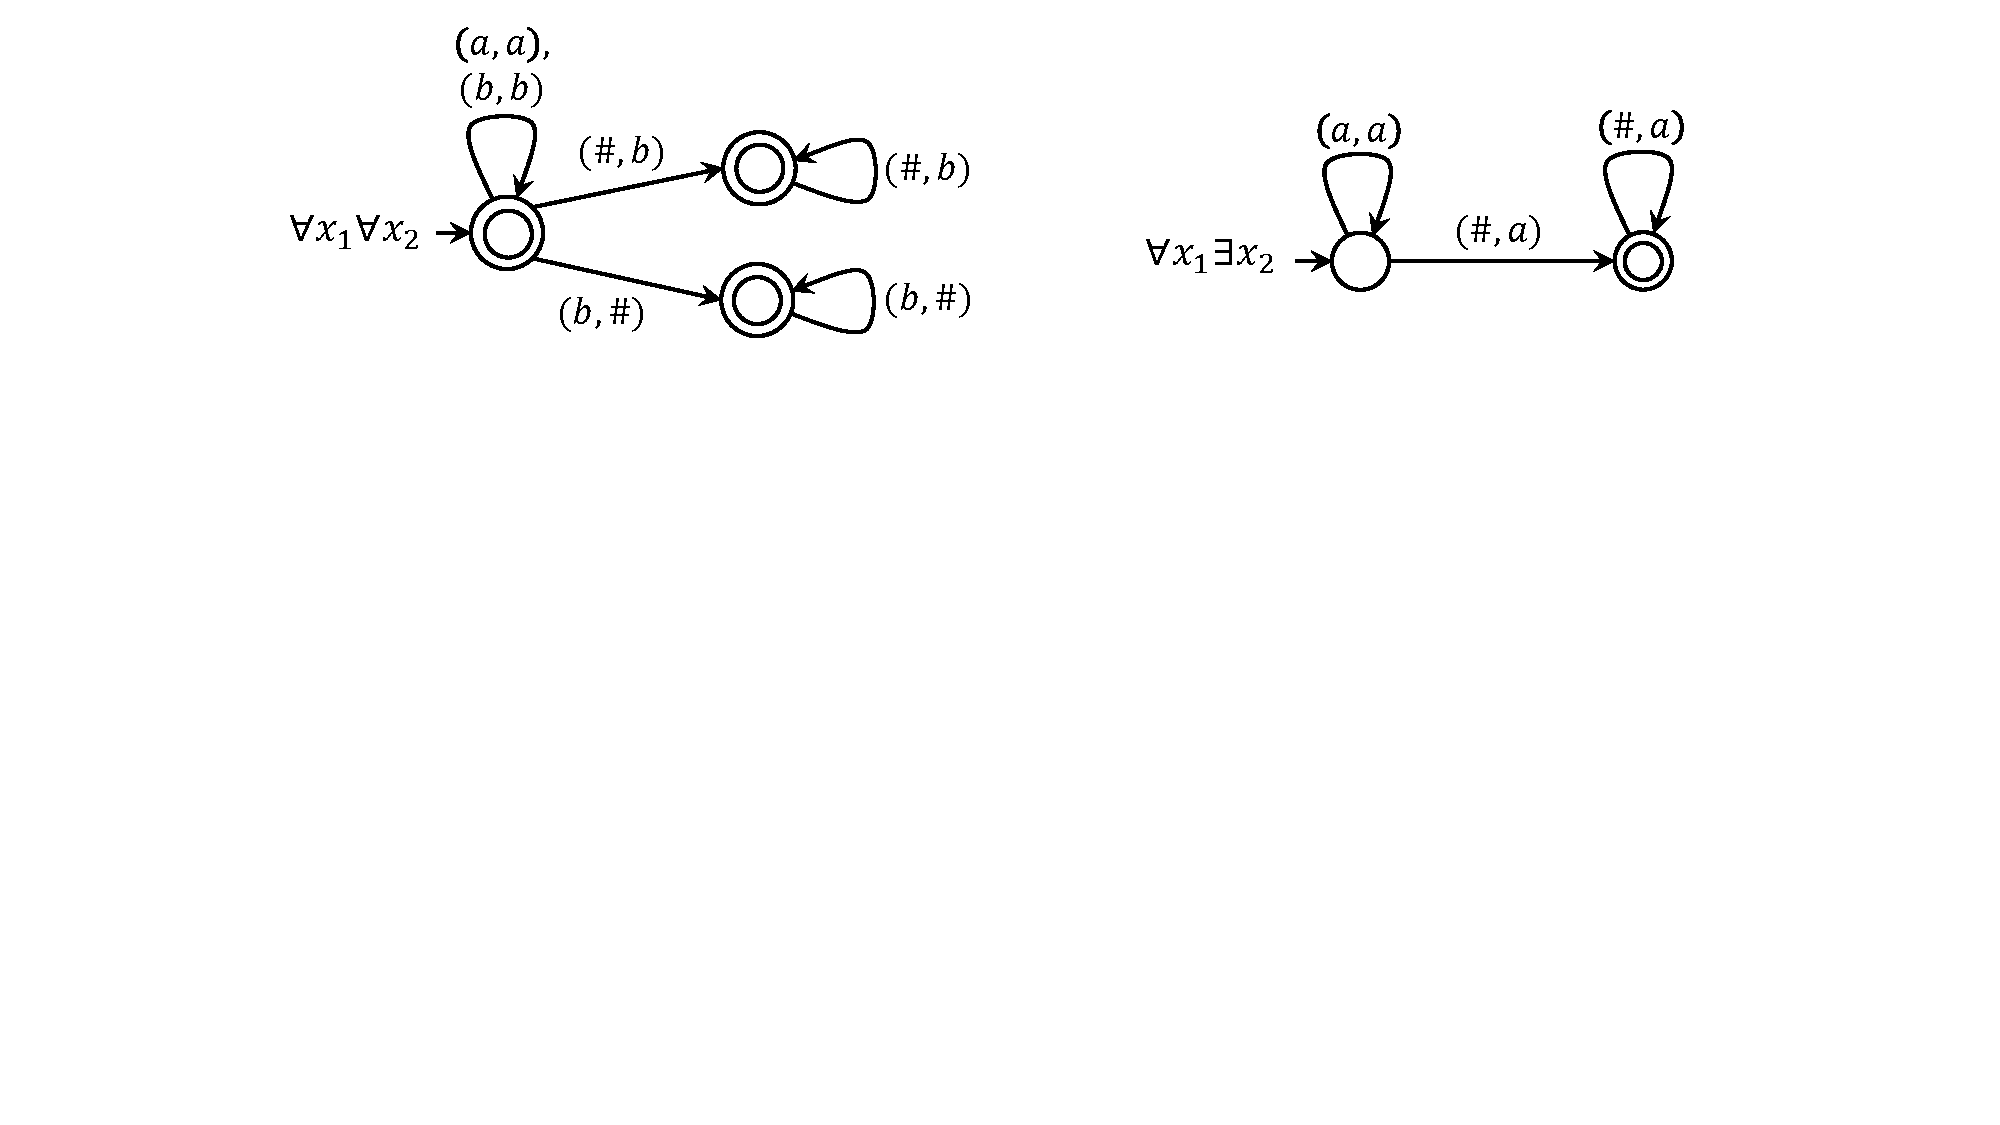
\includegraphics[scale=0.5]{figures/examples.pdf}
    \end{center}
    \caption{The NFH $\A_1$ (left) and $\A_2$ (right).}
    \label{fig:nfh_examples}
%    \hrulefill
\end{figure}


\begin{figure}[ht]
%\hrulefill
    \begin{center}
        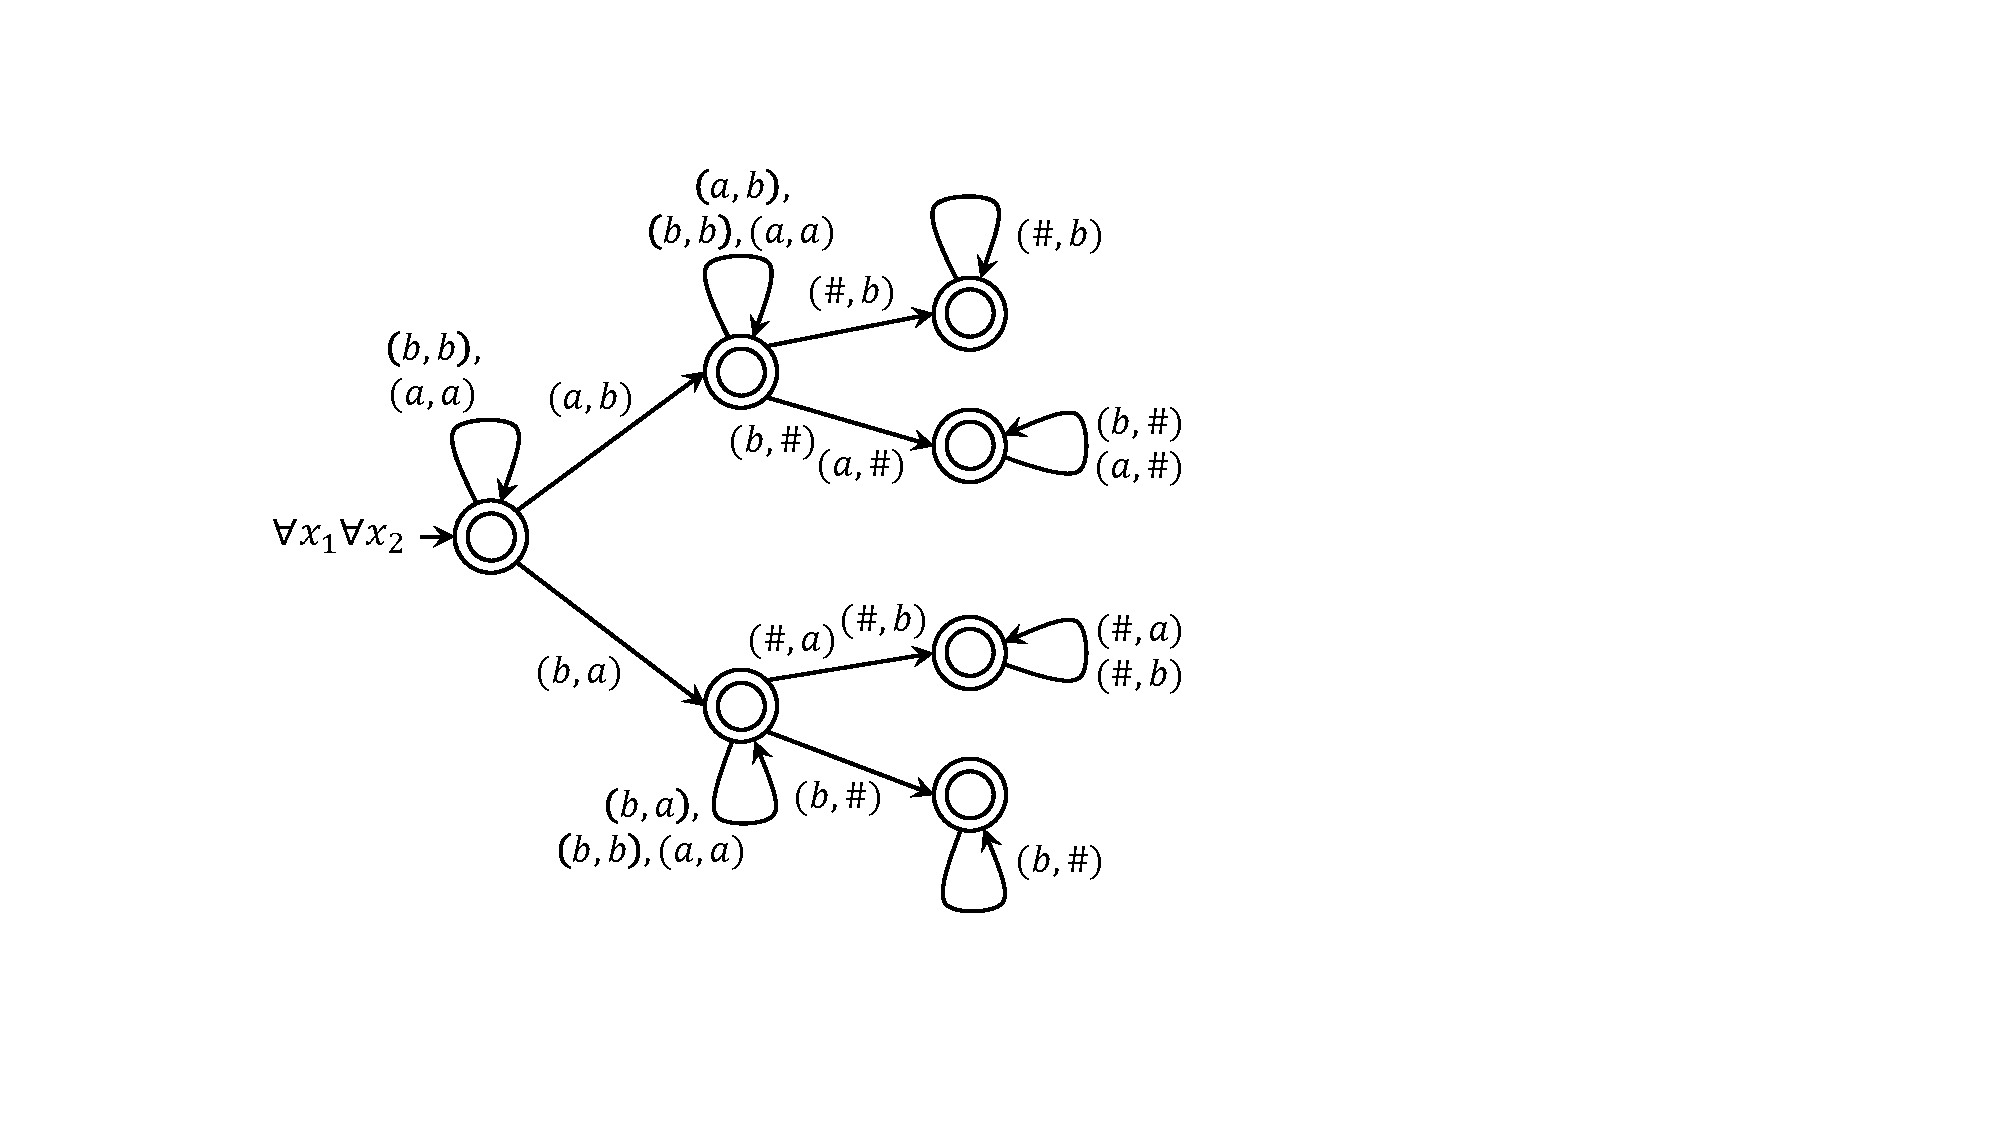
\includegraphics[scale=0.5]{figures/a_implies_a.pdf}
    \end{center}
    \caption{The NFH $\A_3$.}
    \label{fig:ordered}
%    \hrulefill
\end{figure}
\end{example}



We consider several fragments of NFH, which limit the structure of the quantification condition $\alpha$.
$\nfhf$ is the fragment in which $\alpha$ contains only $\forall$ quantifiers, 
and similarly, in $\nfhe$, $\alpha$ contains only $\exists$ quantifiers. In 
$\nfhef$ $\alpha$ is of the form $\exists x_1 \cdots \exists x_i \forall 
x_{i+1}\cdots \forall x_k$, and finally, in $\nfhfe$, $\alpha$ is of the form  
$\forall x_1 \cdots \forall x_i \exists x_{i+1}\cdots \exists x_k$.





%\subsection{Hyperautomata over Hyper-infinite Words}

We now lift the notion of hyperautomata to infinite words. 
A {\em hyper-infinite word} over $\Sigma$ is a set of infinite words over $\Sigma$. 
As before, an automaton $\A$ for a hyperlanguage $\cal L$ consists of an underlying automaton which runs on the tuples of words that are assigned to the word variables of $\A$. In the case of hyper-infinite words, the underlying automaton runs on tuples of infinite words. We consider a B{\"u}chi acceptance condition for the underlying automata. 

\begin{definition}
A {\em nondeterministic B{\"u}chi hyper-word automaton (NBH)} is a tuple $\A = 
\tuple{\Sigma, X=\{x_1,\ldots x_k\}, Q, Q_0, \delta, F, \alpha}$, where all 
elements are as in NFH and acceptance condition defined by the underlying NBW 
of $\A$ is $\hat{\A} = \tuple{\Sigma^k,Q,Q_0,\delta,F}$.

\end{definition}

In particular, consider a hyper-infinite word $S$ and an 
assignment $v:X\rightarrow S$. Then $\hat\A$ accepts $\zip(v)$ iff the run of 
$\hat\A$ on $\zip(v)$ visits some state in $F$ infinitely often. 
The definition of $\models$, acceptance, and $\lang{A}$ are all as in NFH.
As with NFH, we consider the different fragments of NBH$_\forall$, NBH$_\exists$, NBH$_{\forall\exists}$ and NBH$_{\exists\forall}$.



